 %%----------------------------------------------------------------------------------
% SETTING STARTS - DO NOT Change this. It is the required setting A4 page, 11pt, onside print, book style
%%----------------------------------------------------------------------------------
\documentclass[french,a4paper,11pt,oneside]{book}

%%-------------------------------------
%% Page margin settings - % half inch margin all sides (recommended)
%%-------------------------------------
\usepackage[utf8]{inputenc}
\usepackage{babel}
\usepackage[margin=1.2in]{geometry} 

\usepackage{setspace}


%%-------------------------------------
%% Font settings - % CM San or Ariel (recommended)
%%-------------------------------------
% Switch the following two line off: to revert back to default LaTex font (NOT recommended)
\usepackage{amsfonts}
\renewcommand*\familydefault{\sfdefault}

%%-------------------------------------
%% Math/Definition/Theorem/Algorithm packages settings 
%%-------------------------------------
\usepackage[cmex10]{amsmath}
\usepackage{amssymb}
\usepackage{amsthm}
\newtheorem{mydef}{Definition}
\newtheorem{mytherm}{Theorem}

%%-------------------------------------
%% Algorithms/Code Listing environment settings  - 
%% Please do not change these settings
%%-------------------------------------
\usepackage{algorithm}
\usepackage{algpseudocode}
\renewcommand{\algorithmicrequire}{\textbf{Input:}}
\renewcommand{\algorithmicensure}{\textbf{Output:}}
\usepackage[utf8]{inputenc}
\usepackage{listings}
\usepackage{xcolor}
\definecolor{codegreen}{rgb}{0,0.6,0.1}
\definecolor{codegray}{rgb}{0.5,0.5,0.5}
\definecolor{codeblue}{rgb}{0.10,0.00,1.00}
\definecolor{codepurple}{rgb}{0.58,0,0.82}
\definecolor{backcolour}{rgb}{1.0,1.0,1.0}

\usepackage{epsfig}
\usepackage{fancyhdr}
\usepackage{listings}
\usepackage{color}
\usepackage{makeidx}

% Valeurs par défaut le lstset
\lstset{language={},%C,Assembleur, TeX, tcl, basic, cobol, fortran, logo, make, pascal, perl, prolog, {}
    literate={â}{{^a}}1 {ê}{{^e}}1 {î}{{^i}}1 {ô}{{^o}}1 {û}{{^u}}1
         {ä}{{"a}}1 {ë}{{"e}}1 {ï}{{"i}}1 {ö}{{"o}}1 {ü}{{"u}}1
         {à}{{`a}}1 {é}{{'e}}1 {è}{{`e}}1 {ù}{{`u}}1 
         {Â}{{^A}}1 {Ê}{{^E}}1 {Î}{{^I}}1 {Ô}{{^O}}1 {Û}{{^U}}1
         {Ä}{{"A}}1 {Ë}{{"E}}1 {Ï}{{"I}}1 {Ö}{{"O}}1 {Ü}{{"U}}1
         {À}{{`A}}1 {É}{{'E}}1 {È}{{`E}}1 {Ù}{{`U}}1,
    commentstyle=\scriptsize\ttfamily\slshape, % style des commentaires
    basicstyle=\scriptsize\ttfamily, % style par défaut
    keywordstyle=\scriptsize\rmfamily\bfseries,% style des mots-clés
    backgroundcolor=\color[rgb]{.95,.95,.95}, % couleur de fond : gris clair
    framerule=0.5pt,% Taille des bords
    frame=trbl,% Style du cadre
    frameround=tttt, % Bords arrondis 
    tabsize=3, % Taille des tabulations
%    extendedchars=\true, % Incompatible avec utf8 et literate
    inputencoding=utf8,
    showspaces=false, % Ne montre pas les espaces 
    showstringspaces=false, % Ne montre pas les espaces entre ''
    escapechar=°}  % Caractère d'échappement, permet des commandes latex dans la source




%%-------------------------------------
%% Graphics/Figures environment settings
%%-------------------------------------
\usepackage{graphicx}
\usepackage{subfigure}
\usepackage{caption}
\usepackage{lipsum}

%%-------------------------------------
%% Table environment settings
%%-------------------------------------
\usepackage{multirow}
\usepackage{rotating}
\usepackage{makecell}
\usepackage{booktabs}
%\usepackage{longtable,booktabs}

%%-------------------------------------
%% List of Abbreviations settings
%%-------------------------------------
\usepackage{enumitem}
\newlist{abbrv}{itemize}{1}
\setlist[abbrv,1]{label=,labelwidth=1in,align=parleft,itemsep=0.1\baselineskip,leftmargin=!}

%%-------------------------------------
%% Bibliography/References settings   - Harvard Style was used in this report
%%-------------------------------------
\usepackage[hidelinks]{hyperref}
\usepackage[comma,authoryear]{natbib}
\renewcommand{\bibname}{References} % DO NOT remove or switch of 

%%-------------------------------------
%% Appendix settings     
%%-------------------------------------
\usepackage[toc]{appendix}
\usepackage{lmodern}

\newcommand\tab[1][1cm]{\hspace*{#1}}

\newcommand\boit[1]{\textit{\textbf{#1}}}

\newtheorem{definition}{Definition}

%%-------------------------------------
%% Document begins   
%%-------------------------------------
\begin{document}

    \captionsetup[figure]{margin=1.5cm,font=small,name={Figure},labelsep=colon}
    \captionsetup[table]{margin=1.5cm,font=small,name={Table},labelsep=colon}
    \SetLipsumDefault{1}
    
    \frontmatter
    
    \begin{titlepage}      
        \begin{center}
            
\includegraphics[width=3cm]{figures/logo.jpg}\\[0.5cm]
            {\LARGE École supérieure d'informatique - HE2B ESI\\[0.5cm]
            Département des sciences informatiques}\\[2cm]
			%{\color{blue} \rule{\textwidth}{1pt}}
			
			% -------------------------------
			% You need to edit some details here
			% -------------------------------  
            \linespread{1.2}\huge {
                %%%%%%%%%%%%%%%%%%%%%%%%%%%%
                %TODO: 1 TITLE of Your PROJECT 
                %%%%%%%%%%%%%%%%%%%%%%%%%%%%
                % change the following line                
                Protocole Applicatif TCP
            
            }
            \linespread{1}~\\[2cm]
			%{\color{blue} \rule{\textwidth}{1pt}}
            {\Large 
                %%%%%%%%%%%%%%%%%%%%%%%%%%%%
                %TODO: 2 YOUR NAME
                %%%%%%%%%%%%%%%%%%%%%%%%%%%%             
                % chnage the following line
                Basile Routier
                % change end             
            }\\[1cm] 
            

            {\large 
                %%%%%%%%%%%%%%%%%%%%%%%%%%%%
                %TODO: 3 YOUR NAME Supervisor's name(s)
                %%%%%%%%%%%%%%%%%%%%%%%%%%%%             
                % change the following line                
                \emph{Professeur:} M. Bastreghi}\\[1cm] % if applicable
            
    		% PLEASE DO NOT CHANGE THIS TEXT %
            \large Bachelier en \textit{Informatique de Gestion}\\[0.3cm] 
            \vfill
            
            
            \today % Please update this date you can use \date{April 2020} for fixed date
        \end{center}
    \end{titlepage}
    
    % -------------------------------------------------------------------
    % Abstract and Acknowledgement
    % -------------------------------------------------------------------
    
    % \input{chapters/abstract.tex}
    % -------------------------------------------------------------------
	% Acknowledgement
	% -------------------------------------------------------------------
   
    % \input{chapters/acknowledgments.tex}   
    
    % -------------------------------------------------------------------
    % Contents, list of figures, list of tables
    % -------------------------------------------------------------------
    
    \tableofcontents

    %%%%%%%%%%%%%%%%%%%%%%%%%%%%%%%%%%%%%%%%%%%%%%%%%%%%%%%%%%%%%%%%%%%%%%%%
    %%                                                                    %%  
    %%  Main chapters and sections of your project                        %%  
    %%  Everything from here on needs updates in your own words and works %%
    %%                                                                    %%
    %%%%%%%%%%%%%%%%%%%%%%%%%%%%%%%%%%%%%%%%%%%%%%%%%%%%%%%%%%%%%%%%%%%%%%%%
    \mainmatter
    % Read for preparation of document in LaTex 
    % Lamport, L. (1986), LATEX: A Document Preparation System, Addison-Wesley.
    
    \chapter{Introduction}
\label{ch:into} % This how you label a chapter and the key (e.g., ch:into) will be used to refer this chapter ``Introduction'' later in the report. 
% the key ``ch:into'' can be used with command \ref{ch:intor} to refere this Chapter.


\textbf{L'objectif} de ce travail étant de vous présenter en quoi consistent un protocole applicatif dans une infrastructure réseau et les différentes implémentation possible.
Le but étant aussi de vous fournir une 'documentation' permettant à celui ou celle de comprendre le concept qui se trouve derrière et la pratique.
\\

\section{Service et protocole applicatif}

Vous avez peut-être déjà entendu d'un protocole applicatif mais sans réellement comprendre le sens et son utilité.
Un \textbf{protocole applicatif} est une couche se 'superposant' sur une couche d'un protocole réseau tel que TCP ou UDP.

\begin{definition}
  Selon Y. Sennoun. \cite{def_protocol_app}, Un protocole applicatif est un ensemble de règles définissant le mode de communication entre deux applications informatiques. Ils se basent sur les protocoles de transport (TCP/UDP) pour établir dans un premier temps des routes et échanger les données selon l’ensemble des règles du protocole applicatif sélectionné.
\end{definition}

Dans le cas pratique que l'on souhaite donner, cela correspond plus à définir un dialogue et détecter les erreurs qui peuvent arriver au cours d'un échange de message, ...

Le \textbf{"dialogue"} peut changer en fonction de l'utilisation qu'on souhaite faire de l'application et des différents moyens de communications.


    {
    \centering
    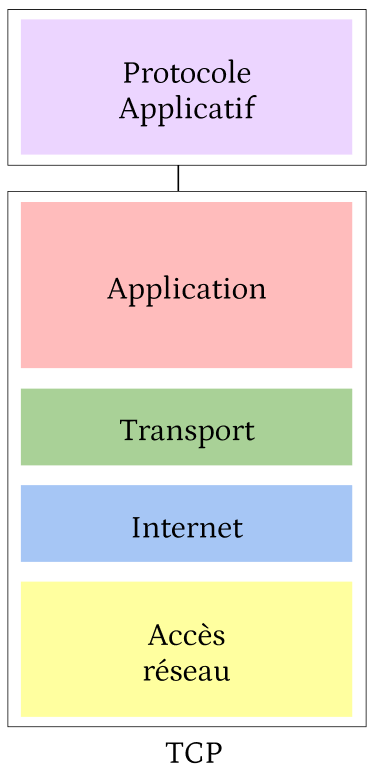
\includegraphics[width=5cm]{figures/protocole-appli.png}
    \par
    }

Avant de découvrir cela, 
Pour créer un protocole applicatif, il faut \emph{impérativement} passer par l'utilisation de socket permettant la création d'un canal de communication. \textbf Il faut toute fois définir quel mode souhaite on utilisé :
\begin{itemize}
     \item \textbf{Mode connecté}
     \item \textbf{Mode non connecté (datagram)}
\end{itemize}

Ces deux modes sont bien différents l'un de l'autre, nous le verrons plus tard.

\section{Utilité d'un protocole applicatif}

Il y a différentes utilité d'implémenter un protocole applicatif sur un réseau, serveur tel que :
\begin{itemize}
     \item Le contrôle du trafic comme on le souhaite
     \item La vérification et détection des erreurs
     \item Flexibilité en fonction du cas d'utilisation
     \item Le serveur est sécurisé si bien configuré
\end{itemize}

Cela est principalement utile pour avoir un certain contrôle sur le flux qui est envoyé et détecter les problèmes qui peuvent arriver lors d'envoie sur le réseau.


    \chapter{Configuration des différents protocoles}

Le but principal de ce chapitre étant d'abord de \textbf{comprendre} et 
\textbf{réaliser la configuration} du protocole applicatif qu'on souhaite. 

Le premier problème étant que pour pouvoir le définir et le configurer, il faut déjà savoir quel protocole réseau souhaite-on utiliser. 
C'est ce que nous allons voir dans la section suivante qui sera très brève.

\section{Protocole réseau}

Le protocole de transport de paquet est un élément essentiel dans notre cas d'utilisation car permet la transmission de paquet d'un client/serveur vers un serveur/client. Sans cela notre protocole applicatif n'aurait aucun sens et ne serait en aucun cas utile. Mais nous ne survolerons que les bases de ceux-ci sans rentré dans les détails.

\subsection{TCP}

Le protocole de contrôle de transmission (TCP) est un protocole de transport qui est utilisé au-dessus du protocole IP pour assurer une transmission fiable des paquets.
\\
Il permet la résolution d'un grand nombre de problèmes liés à la messagerie par paquets, tels que les paquets perdus, les paquets hors d'usage, les paquets en double et les paquets corrompus.
\\
TCP fonctionne comme des feux de signalisation pour les voitures, il fait attention que les paquets non pas "d'accident" entre eux.
D'autres détails sont aussi important dans TCP mais ne sont pas important dans le cadre du protocole applicatif souhaité.
Si besoin de très bon livres (mis en bibliographie) explique les détails de ceux-ci.

\subsection{UDP}

Le User Datagram Protocol (UDP) est tout comme TCP un protocole de transport de paquet mais à quelques spécificité tel que le transport rapide des paquets utilisé principalement pour l'affichage en temps réel (vidéo, appel, ...). Il a le même principe que TCP sans les contraintes de "feux de signalisation" pour les paquets.
Comme dis précédemment, si vous avez besoins de plus de détail les livres sont vos amis.

\subsection{Utilisation}

Commençons par définir quel type de protocole de transport souhaite-on utiliser. Dans notre cas pratique, nous utiliserons le TCP qui permet comme cité :
\begin{itemize}
    \item Le faite d'être sûr et certains de recevoir notre paquet (message)
    \item Avoir notre paquet trié dans l'ordre dans lequel il a été envoyé
\end{itemize} \hfill \\ \par

Tandis que UDP est pour la plupart du temps utilisé pour l'envoie de donnée en temps réel. Par exemple, des jeux vidéos, streaming, appel wifi. \\ \par

C'est pour cela que dans NOTRE cas, tcp est utile car nous enverrons des messages et des fichiers. Et ceux-ci ne doivent pas pouvoir subir de perte de paquet. Ce qui arriverait certainement avec UDP.


\underline{\textbf{Création d'un point de communication TCP pour l'écoute :}}
\begin{itemize}
    \item Création d'un point de communication (socket)
    \item Fourni un nom à une socket (bind)
    \item Attente des connexions sur une socket (listen)
    \item Accepter le client (accept)
    \begin{itemize}
        \item Dans notre exemple, nous n'allons pas réaliser cette étape car elle est utilisé par la suite
        \item Revenir à l'étape d'attente une fois la connexion établie
    \end{itemize} 
\end{itemize}
Comme dis précédemment, ici nous nous intéressons que très peu à la création de socket et les autres fonctionnalités de celui-ci. C'est pourquoi l'ensemble du code est écrit si joint avec quelques brèves explications. \\ \\

\underline{createSocket.c :}
\lstinputlisting{codes/createSocket.c}

\underline{Explications de certains détails :}
\begin{lstlisting}
    socket() :
        AF_INET -> est le protocole pour IPV4
        SOCK_STREAM -> on demande d'utiliser du TCP
    bind() :
        On donne un nom a la socket 
        (avec la famille IPV4, le nom de port et l'adresse IP courante)
    listen():
        On specifie simplement le nombre de connexion maximum 
        qu'il peut y avoir en attente.
\end{lstlisting}

\section{Protocole applicatif côté serveur}

Comme vous avez pu le comprendre un protocole applicatif est superposer dans à la couche TCP, utile pour vérifier les problèmes qui peuvent survenir et/ou définir un dialogue entre deux machines à état . \\ \\

L'important étant d'établir un dialogue en fonction de ce qu'on souhaite faire de l'application. Dans notre cas, nous allons créer un protocole qui :
\begin{itemize}
\item Permet de vérifier et lire la longueur exact du message
\item Vérifier si un client s'est déconnecté
\item A la capacité de vérifier si il y a une erreur dans le message envoyé
\item Compatibilité au niveau du client
\item Permet de vérifier et lire le type du message (message/fichier)
\end{itemize}

Le protocole au niveau théorique étant maintenant défini, il nous reste à nous intéresser sur : comment pouvoir l'implémenter du côté serveur. \\ \\



\subsection{Lecture message d'une taille précise}

\par 
Lors de l'envoi d'un message d'un client/serveur à un serveur/client, celui-ci \textbf{ne peut pas deviner la taille du message}, c'est pour cela que nous allons définir une règle permettant de ne pas lire un nombre prédéfini de byte(s) mais le nombre exact. \\ \\ \par
Cette règle est la suivante :
\begin{itemize}
\item Notre message devra contenir un "header" qui va contenir 4 bytes avec l'information sur la taille du message. Qui sera mis sous format de \boit{nombre pour faciliter le formattage côté serveur}
\begin{itemize}
\item Si celle-ci ne contient pas la taille, une erreur est déclenché
\item Si la taille correspond bien au nombre de byte(s) présent et qu'il y a correctement le nombre de byte(s) reçu alors nous pouvons lire le message
\end{itemize}
\item Dans notre cas, on va aussi résoudre les règles suivantes tel que :
\begin{itemize}
\item Vérifier si un client s'est déconnecté
\item Vérifier si il y a une erreur dans le message envoyé
\end{itemize}
\end{itemize}

\hfill \\ \par Pour ne pas \textbf{bloquer} le processus parent avec des appels systèmes qui pourrait être bloquant, nous allons \textbf{utiliser la création de fils}. 
Bien sûr cette partie n'est pas obligatoire pour faire un protocole applicatif mais apporte une touche en plus. Avec : \begin{lstlisting}
    int fork()
\end{lstlisting}

Renvoyant le PID du fils est renvoyé au processus parent, et 0 est renvoyé au processus fils. Sinon renvoye -1 en cas d'erreur.

Fork va créer un fils qui aura comme parent notre programme. Lui permettant de faire appel au fonction ou appel système en dehors de notre processus courant.


\lstinputlisting{codes/tcpserver.c}

Nous utilisons certains appels systèmes :

\begin{lstlisting}
    Accept() : Permettant d'accepter un client ce trouvant dans la liste d'attente 
    quand le socket ecoute sur son port.

    Signal() : Permettant de réaliser une certaine action sur un signal reçu.
\end{lstlisting}

Pour palier au processus zombie (un processus attend que son père l'appel pour pouvoir finir le processus), nous utiliserons l'appel système signal qui nous permet d'ignorer le processus zombie et donc le rendre orphelins. \\ \par

La fonction : \begin{lstlisting}
    void displayClientConnection(struct sockaddr_in client_addr);
\end{lstlisting}

Affiche simplement les informations du client grace à la structure sockaddr in.

Et  \begin{lstlisting}
    void receiveMessageClient(int sockli);
    // Qui sera la fonction contenant les regles de notre protocole applicatif
\end{lstlisting} \hfill \\ \par

Comme nous decidons de creer un fils, nous devons utiliser une technique
pour pouvoir ignorer le signal du fils et qu'il devienne orphelins.

Il faudra \textbf{prendre en compte} plusieurs informations complémentaires dans l'implémentation de notre protocole applicatif, tel que :
\begin{itemize}
    \item La récupération d'information sans toucher au message
    \item Vérifier qu'un client ne s'est pas déconnecté en cours de route
    \item Faire en sorte de pouvoir utiliser telnet (ou d'autres clients)
    \item Analyse syntaxique
\end{itemize}

\textbf{Remarque :}
    L'utilisation de telnet est simplement une \textbf{fonctionnalité} supplémentaire ajouté à mon code qui RETIRE le control sequence (CRLF (Line Feed et Carriage Return)). \\  \par
    

 \textbf{Voici plusieurs images représentants notre protocole applicatif courant mise en place et comment celui-ci fonctionne.} \\ \par

Pour l'instant notre protocole est assez minimaliste pour ne pas avoir qu'un seul bloque vous décrivant l'entiéreté du protocole. Le but étant de garder un schéma simple au départ puis l'agrandir au fur et à mesure. \\ \\ \\ \\ \\ \\ \\ \\ \\ \\ \\ \\ \\ \par


    {
    \centering
    \textit{Communication Client vers Serveur} \\
    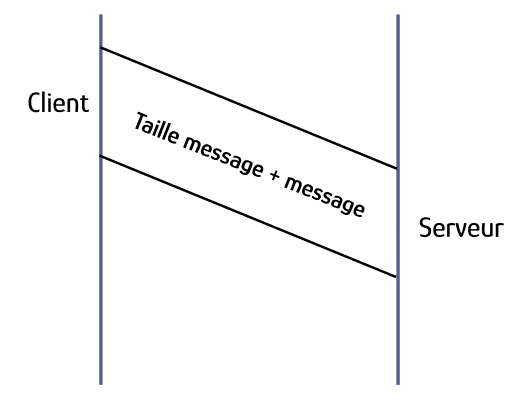
\includegraphics[width=10cm]{figures/cl_serv.png}
    \par
    }
Dans cette exemple :\\ 
    \tab[2cm] Le client envoye un message au serveur avec la taille du message (sur 4 bytes). Ce message contient des charactères sous format de nombres et non de lettre ou autres pour permettre un formattage plus simple côté serveur et le reste du message. \\ \par \boit{\underline{Une idée du type de message ce trouve après l'arbre de décision}}\\ \par


\textit{Arbre de décision permettant de savoir quand un message passe ou pas.} \\ \par
    {
    \centering
    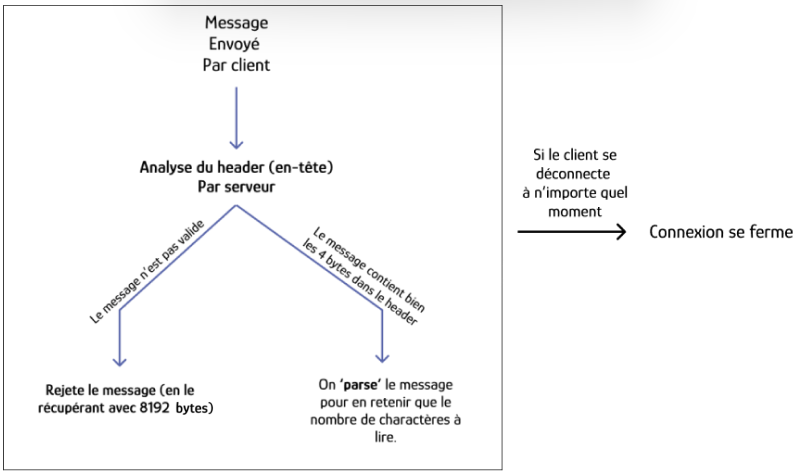
\includegraphics[width=18cm]{figures/arbre_head_4bytes.png}
    \par
    }

    Un nombre = un charactère = 1 byte. On peut simplement distinguer qu'un nombre est bien un nombre avec une fonction qui analyse le charactère. Il faudra simplement analyser les 4 bytes de début pour vérifier que ce sont bien des nombres et pas autres choses. \\ \par

    Dans notre protocole applicatif, nous décidons qu'un message reçu ne peut \textbf{PAS} dépasser 8192 bytes. Donc si un message est mal formé ou invalide, nous décidons par précotion de supprimer l'entiereté du contenu du buffer. \\ \par

    \boit{ATTENTION :} \par
    En cas de problèmes car nous supprimons une partie/l'entiéreté du contenu du buffer en mémoire. Et dpnc peut-être un message lu n'appartenant pas au destinataire aurait pu être supprimé. \par
    Dans notre protocole, nous n'avons pas défini de sécurité particulière pour vérifier les messages pouvant avoir des 'gros' problèmes. Tel que (\underline{ceci ne sont que des idées}) :
    \begin{itemize}
        \item Le faite de pouvoir supprimer le nombre exact même en ne connaissant pas le nombre de charactère (en ajoutant charactères spéciaux à la fin)
        \item Rajouter au début d'un message l'id d'un utilisateur
    \end{itemize}
    On pourrait donc envisager le faite de mettre un charactère de fin pour pouvoir supprimer le nombre exact de charactère. \\ \\ \par
    

    Pour réaliser l'analyse de l'entête, nous allons utiliser l'appel système :
    \begin{lstlisting}
        recv(socketClient, buffer, 4, MSG_PEEK) -> renvoie -1 si un probleme arrive
        tel que : la deconnexion brutale d'un client (sans prevenir)
    \end{lstlisting}
    Nous savons que nous devons lire \textbf{seulement 4 bytes} pour récupérer le header et utilisons le flag MSG PEEK pour :
    \begin{itemize}
        \item récupérer le message sans le supprimer et pouvoir l'analyser.
        \item Vérifier qu'un client ne s'est pas déconnecté brutallement.
    \end{itemize} \hfill \\



    \textbf{Pour l'analyse du message : } \par
    Il faudra lire \textit{charactère par charactère} et vérifier si il est un chiffre.\par
    Puis vérifier si le nombre de chiffre correspond à celui qu'on attend. \\ \\ \par

    Voici comment est analysé un message lors de la réception du message. 

    {
    \centering
    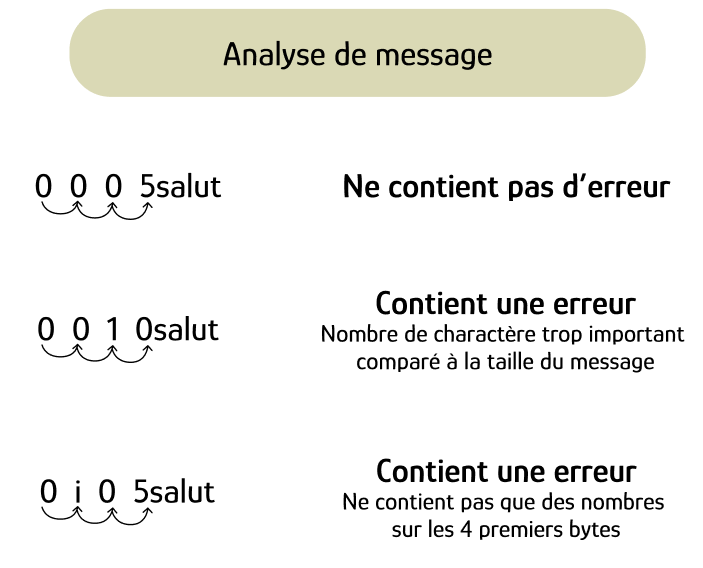
\includegraphics[width=7cm]{figures/msg_4bytes_ana.png}
    \par
    }

    
    Le message est analysé au départ pour \textbf{seulement vérifier} si il contient bien 4 bytes de chiffres au début du message. \par
    
    \tab[1cm]1. Après analyse du message, on 'parse'le message pour à ce moment vérifier si le 
    \tab[2cm]nombre de charactères est bien celui du nombre de bytes lus. \par

    \tab[2cm]- \textit{Nous faisons ca pour une \textbf{meilleure décomposition} du code} \\ \\

    
\subsection{Récupération du message après analyse}

Passons à \textbf{la récupération du message après analyse} permettant de lire un message reçu.

Bien évidemment, il est important de connaitre comment fonctionne la réception d'un message. C'est pour cela que je  vais faire un bref résumé sur le fonctionnement de celui-ci. \\ \par

Malheuresement TCP, ne gère seulement que les données et non pas les paquets. Ce qui signifie que si plusieurs paquets arrive dans le buffer, notre appel système recv() recevra la taille indiqué (ce qui peut créer une fuite de donnée). \\ \par


C'est pour cela que nous avons réalisé une couche applicative pour éviter ce genre de problèmes. En par exemple :
\begin{itemize}
    \item \textbf{Limitant le nombre de bytes maximums à recevoir d'un message}
    \item \textbf{En donnant un header pour savoir le nombre de byte à lire}
\end{itemize}

Parenthèse faite, reprenons sur la lecture du message grâce à sa taille.

Nous avons un message type :

\begin{lstlisting}
    0005salut
\end{lstlisting}

Pour pouvoir récupérer le message, nous allons récupérer les chiffres contenus dans le header et les convertir \textbf{pour pouvoir} recevoir le reste du message d'une longueur défini. \\ \\ \par

    {
    \centering
    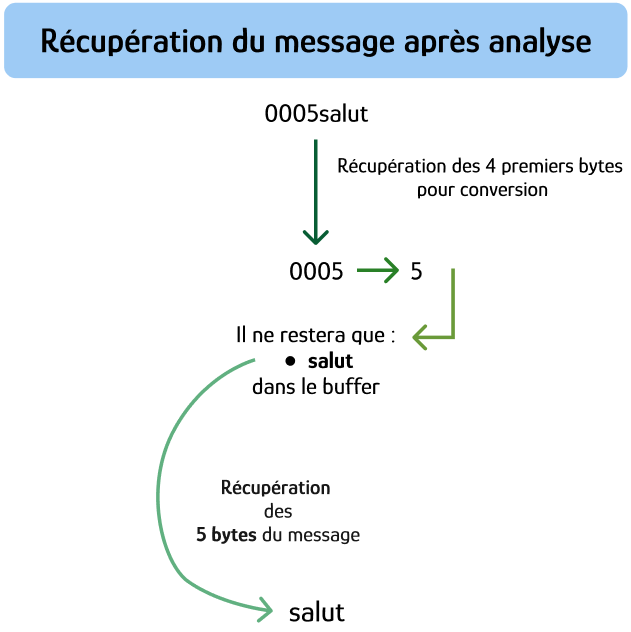
\includegraphics[width=10cm]{figures/recup_message_ana.png}
    \par
    } \hfill \par

    Comme vu précédemment, nous n'avons pas supprimé le header grâce à aux flag : \begin{lstlisting}
        MSG_PEEK -> permettant de regarder le message sans en supprimer son contenu
    \end{lstlisting}

    On souhaite récupérer la taille du message, mais le \textbf{souci étant que ce ne sont que des charactères}.\par C'est pour cela qu'on devra convertir l'ensemble des charactères en chiffre. \\ \\ \par

    On récupère le message avec la taille converti précédemment. Ici, nous récupérons \textbf{5 bytes} du message avec le flag :
    \begin{lstlisting}
        MSG_PEEK
    \end{lstlisting} \hfill \\

    {
    \centering
    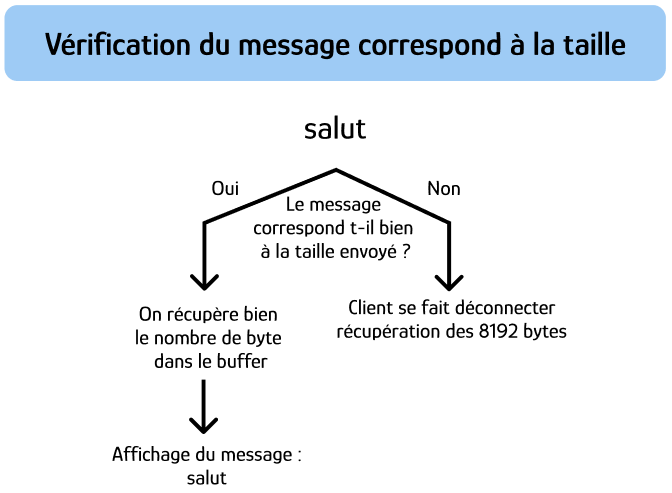
\includegraphics[width=12cm]{figures/recup_message_entier.png}
    \par
    } \hfill \par

    Dans notre cas, si le message ne correspond pas \underline{EXACTEMENT} à la taille qu'il a envoyé (qu'il soit plus court ou plus long), celui-ci sera déconnecté.

    Comme dans notre cas, un message ne \textbf{POURRA JAMAIS} dépassé 8192 bytes, nous pouvons savoir qu'il ne sera jamais plus long que ce qu'il prétend. Voir début sous chapitre "Lecture message d'une taille précise" page 5.
    

    Voici notre premier protocole applicatif fait et appliquer sur l'ensemble de notre serveur.

    On rajoutera \textbf{par la suite} une couche en plus à notre protocole applicatif, nous \textit{permettant de recevoir des fichiers}. \par 
    Ce qui modifiera légéremment certains aspects que nous avons vu précédemment. \\ \\ \\



\subsection{Ajout fonctionnalité fichier}

Pour l'instant notre protocole applicatif ne permet \textbf{QUE l'envoie} de message du côté client vers notre serveur. Et donc un protocole assez simple... \par
L'envoie de fichier, de GIF, d'images, etc... devient de plus en plus connues et utilisés au fur et à mesure du temps (c'est presque devenu essentiel). \\ \par
Nous allons donc \textbf{implémenter une fonctionnalité d'envoie de fichier} ce qui modifiera notre protocole applicatif. Un fichier est simplement qu'un ensemble de byte(s) avec un nom pour identifier le fichier et son contenu. \\ \\

Notre protocole applicatif contient pour l'instant un header de \textbf{4 bytes} avec simplement le nombre de byte à lire du message. On souhaiterait le modifier pour qu'il arrive à prendre :
\begin{itemize}
    \item Le nom du fichier
    \item Puis le contenu de celui-ci
    \item Et enfin la fin du fichier
\end{itemize} \hfill \\ \par

C'est pour cela qu'on va 'reinventer' notre protocole pour pouvoir supporter cela. \\ \par

    {
    \centering
    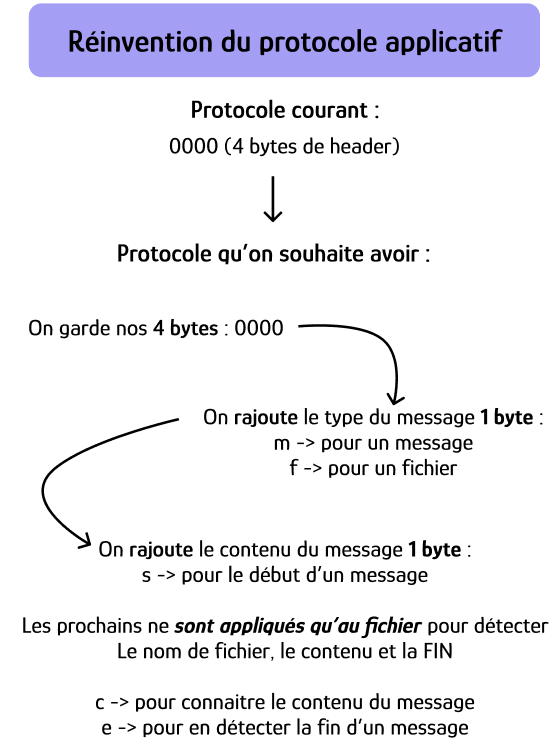
\includegraphics[width=10cm]{figures/reinvention_protocole.png}
    \par
    } \hfill \par

Voici à quoi ressemble le protocole applicatif \textbf{après} l'avoir appliqué à un message envoyé sur les deux type que nous avons. 

    {
    \centering
    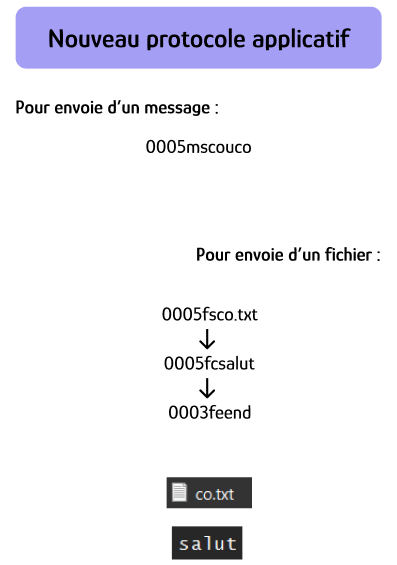
\includegraphics[width=6cm]{figures/new_protocole_applicatif.png}
    \par
    } \hfill \\ \par

Nous allons simplement redevoir \textbf{TOUT} formatter pour pouvoir analyser chaque élément du message et pouvoir en connaitre le type du message et son contenu. Il faudra bien évidemment faire des vérifications pour tester des cas de mauvaise utilisation. \\ \par

Pour la réception du fichier, cela est un peu plus complexe. Voici un format qu'on pourrait utilisé pour la réception de fichier.

    {
    \centering
    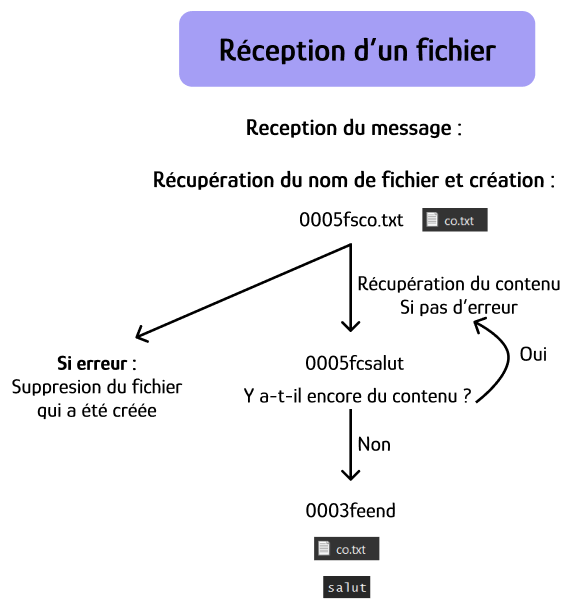
\includegraphics[width=10cm]{figures/reception_fichier.png}
    \par
    } \hfill \\ \par

Pour connaitre si nous avons une suite et si tout est correct, nous devons \textbf{lire sans supprimer le prochain message si il est disponible}.

Nous utilisons de la récursivité (appel à la même fonction) pour ne pas devoir réécrire des conditions en plus qui sont déjà fixés (en utilisant des conditions et des boucles qui ne sont pas super dans ce genre de cas).

    \chapter{Configuration du côté client}

Le côté client est une partie toute aussi importante que notre côté serveur parce qu'elle nous permet d'envoyer des paquets vers le serveur et vérifier si la configuration de notre protocole applicatif à fonctionner.

\subsection{Alternative possible avant de coder pour vérifier protocole applicatif}

Comme j'ai pu le dire précédemment, nous pouvons avant de coder notre côté client utiliser des utilitaires \textbf{permettant de vérifier} si notre protocole applicatif ne rencontre aucun souci 'visible' (car nous devrons envoyer l'ensemble de la requête à la main). \\ \par

Ce genre de manipulation peut avoir plusieurs \textbf{bienfait} mais aussi quelques \textbf{désavantages} : \\ \par

\boit{Avantages} :
\begin{itemize}
    \item Tester notre côté serveur au fur et à mesure sans devoir coder notre client en même temps
    \item Pouvoir détecter les erreurs
\end{itemize} \hfill \\ \par

\boit{Inconvénient} :
\begin{itemize}
    \item Problèmes de sécurité (car nous permettons une application tierce de se connecter)
    \item Pourrait trouver une faille dans le protocole et l'exploiter
    \item Il faut gérer les caractères de fin envoyé par certains protocole du côté serveur (CRLF qui correspond au caractères de fin de line (Carriage Return Line Feed))
\end{itemize} \hfill \\ \par

Voici à quoi ressemblerait une requête envoyé avec \textit{Telnet} vers le serveur :

    {
    \centering
    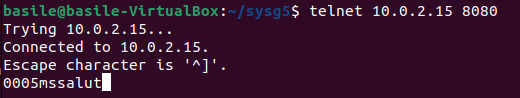
\includegraphics[width=18cm]{figures/example_telnet_conn.png}
    \par
    } \hfill \\ \par

Il faut bien évidemment donner l'adresse IP + le port à la commande :
\begin{lstlisting}
    telnet IpAdress Port
\end{lstlisting}

Nous encodons à la 'main' l'envoie du message mais contenant notre protocole vu que notre prochaine application fera ca pour nous tout à l'heure.

\subsection{Notre côté client, création socket}

Notre application devra se connecter à notre serveur pour cela, on devra comme le serveur de :
\begin{itemize}
\item Créant un point de communication (Socket)
\item Rentrer les informations du serveur dans une structure (sockaddr in) pour définir où et comment se connecter
\item Se connecter  au point de communication via Connect
\end{itemize}

\lstinputlisting{codes/createSocketClient.c} \hfill \\ \par

Nous utilisons des appels systèmes assez importants pour la connection. Bien évidemment certains d'entre eux, on déjà pu être vu comme : socket()

\begin{lstlisting}
    connect(socketfd,(SA*)&server_addr,sizeof(server_addr)
    Nous devons specifie a quel socket se connecter (c'est pour cela que nous avions 
    rentre les informations du serveur).
    En plus de ca, nous fournissons une structure qui permet de stocker 
    les informations de celui-ci.
\end{lstlisting} \hfill \\ \par

Nous pouvons commencer à envoyer si nous souhaitons des informations au serveur grâce à l'appel système : send() que nous verrons plus tard.

\subsection{Notre côté client, envoie de message}

Nous devons définir plusieurs choses avant de commencer à réaliser l'envoie de message. \\ \par

\begin{itemize}
\item Définir notre type d'envoie courant (soit un message (s) ou un fichier (f))
\item Définir le contenu d'envoie courant (si c'est le début, le milieu ou la fin comme défini dans le côté serveur)
\item Créer des fonctions qui retourne la taille d'un message et le stock (la partie code se trouve en annexe si besoin), et correspond à notre côté applicatif
\end{itemize}\hfill \\ \par

Une fois que tout ca est fait, nous pouvons passer à l'envoie de message via l'appel système \textbf{send} :
\begin{lstlisting}
send(socket, message, tailleMsg, flag)
Nous donnerons le socket stocke et renvoyer precedemment, le message contenant
notre protocole applicatif dedans et la taille de celui-ci.
Le flag ne nous interesse pas dans notre cas.
Voici un exemple :
send(socketfd, message, strlen(message),0)
\end{lstlisting}

Le 0 dans le flag est l'équivalent de donné aucun paramètre à notre fonction. \\ \par

Nous allons illustrer ca sous forme de dessin la sélection et l'envoie. \\ \\

\textit{Choisir le mode d'envoie qu'on souhaite} :

    {
    \centering
    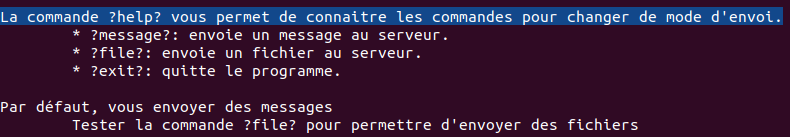
\includegraphics[width=18cm]{figures/selection_type_client.png}
    \par
    } \hfill \\ \par

    Si nous décidions de changer de \textbf{MODE} cela modifirait le type de contenu qu'on souhaite envoyé : \par
    \tab[2cm]Si notre type était avant et après:
    \begin{lstlisting}
        currentCommand='m' et qu'on souhaiterait changer vers l'envoie de fichier (qui se fera plus tard)
        currentCommand='f'
    \end{lstlisting}

    Il faudra bien évidemment vérifier si le serveur n'a pas eu de 'soucis' et à crasher ou vous a déconnecter. Pour cela, on utilise l'appel système : recv avec le flag MSG PEEK \\ \par

    On peut donc passer à la réel lecture au clavier...

    {
    \centering
    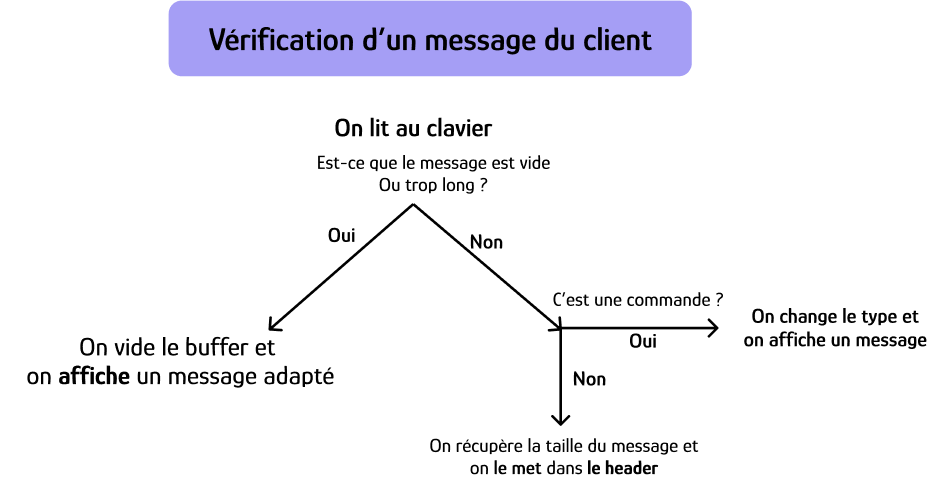
\includegraphics[width=14cm]{figures/verif_msg_client_send.png}
    \par
    } \hfill \\ \par

    Nous avons vérifier et implémenter une partie du header (les 4 bytes pour définir la taille du message), il nous reste simplement qu'à vérifier le \textbf{TYPE de message} qu'on souhaite envoyé et remplir le header pour matcher avec notre protocole applicatif. \\ \par

     {
    \centering
    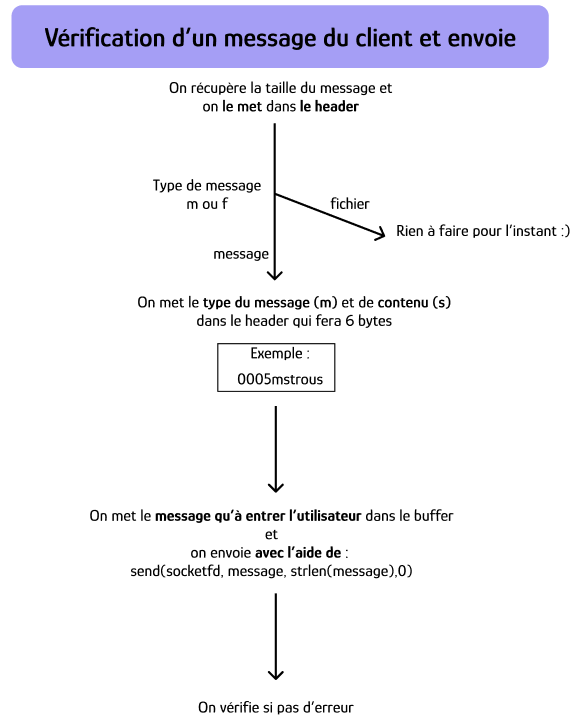
\includegraphics[width=11cm]{figures/verif_msg_client_next.png}
    \par
    } \hfill \\ \par

    Voila notre envoie de message fait en vérifiant les cas pouvant engendrer des erreurs. \\ \par\textbf{N'OUBLIEZ PAS, il est important de vérifier si un appel système à retourner une erreur}

\subsection{Notre côté client, envoie de fichier}

Comme précédemment dis, l'envoie de fichier ou bien même d'autres fonctionnalité sont de plus en plus développé. \\ \par

Un fichier est concrètement qu'un ensemble de bytes. Il suffit donc de récupérer ses bytes et les envoyés au fur et à mesure. \\ \par

Pour l'envoie de fichier, le schéma sera légérement modifiés à celui précédemment. \\ \par

Notre fichier qui sera envoyé aura des header différents en fonction de l'endroit ou ou se trouve :
\begin{itemize}
    \item Si on envoie notre nom de fichier. On enverra fs (fichier start)
    \item Si on envoie le contenu du fichir. On enverra fc (fichier continue)
    \item Si on est a la fin du fichier (pour pouvoir au serveur d'enregistrer le fichier). On enverra fe (fichier end)
\end{itemize}

    {
    \centering
    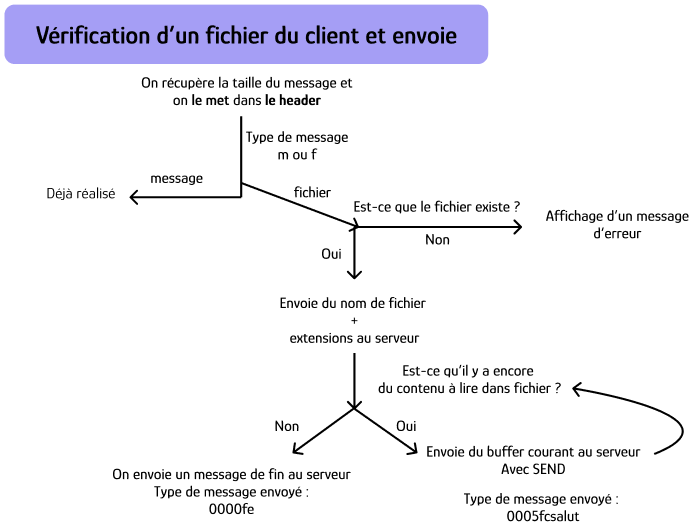
\includegraphics[width=13cm]{figures/verification_fichier_client_envoie.png}
    \par
    } \hfill \\ \par

    Comme dis au dessus, nous passons par des phases dans l'envoie du fichier vers notre côté serveur. Permettant à notre serveur, de savoir à quel endroit nous sommes dans notre fichier.

    Voici la fin de notre côté client qui permet un protocole applicatif plus ou moins riches en fonctionnalité et permet de vérifier les erreurs.
    \chapter{Conclusion}

Un protocole applactif est l'un de ses ensembles de règles permettant à un serveur de pouvoir assurer une certaine sécurité et de vérification des paquets envoyés. Sans celui-ci, les sites internet permettant la retransmission d'informations n'aurait pas su voir le jour. \\ \par

La transmission d'informations tel que les messages, les fichiers, les gifs, et pleins d'autres fonctionnalités sont maintenant omniprésents dans nos vies et sans cela nous ne pourrions plus discuter, ... C'est pour cela qu'un protocole applicatif est fait, gérer différentes fonctionnalités en essayant de limiter le nombre d'erreurs le maximum possibles.

Dans notre protocole applicatif mise en place, pas mal de sécurités et vérifications sont à revoir pour que notre protocole applicatif puisse fonctionné sans que des 'grosses erreurs' arrivent. Nous pouvons citer notemment :
\begin{itemize}
    \item L'envoie de fichier, nous vérifions pas si une personne envoie un fichier trop gros
    \item L'envoie de message, nous définissons 8192 bytes pour l'envoie max de message, le problème étant que si pleins de messages arrivent en même temps sur le serveur. Celui-ci pourrait lire plusieurs messages en même temps et donc causé d'énormes soucis.
    \item Nous ne donnons pas de clé unique à un utilisateur ce qui peut causé des problèmes dans la lecture d'un message (on croit lire un message venant de x mais c'est le message de y).
\end{itemize}

Toutes ses règles peuvent bien évidemment être rajouté au protocole applicatif et donc permettre une meilleure sécurité de celle-ci...

Ne passons pas outre notre protocole réseau, le TCP que nous avons utilisé pour la garantie des messages et le trie de celui-ci. Chaque protocole réseau à des avantages et des inconcivénients. Chacun doit être choisi en fonction de ce que vous souhaiteriez réalisés.
    \chapter{Bibliographie}

  % -------------------------------------------------------------------
    % Bibliography/References  -  Harvard Style was used in this report
    % -------------------------------------------------------------------
    \nocite{*}
    \bibliographystyle{resources/IEEEanot}
    \bibliography{resources/references}

  
    % -------------------------------------------------------------------
    % Appendices
    % -------------------------------------------------------------------
    
    % \begin{appendices}
    %     \input{chapters/appendix_A.tex}
    %     \input{chapters/appendix_B.tex}
    % \end{appendices}
    
\end{document}
